% Copyright (C) 2008 Dominik Dahlem <Dominik.Dahlem@gmail.com>
%
% This file is free software; as a special exception the author gives
% unlimited permission to copy and/or distribute it, with or without
% modifications, as long as this notice is preserved.
%
% This program is distributed in the hope that it will be useful, but
% WITHOUT ANY WARRANTY, to the extent permitted by law; without even
% the implied warranty of MERCHANTABILITY or FITNESS FOR A PARTICULAR
% PURPOSE.

\documentclass[12pt,a4paper]{article}
\usepackage{fancyhdr}
\usepackage[T1]{fontenc}
\usepackage[latin1]{inputenc}
\usepackage{graphicx}
\usepackage{hyperref}
\usepackage{prettyref}
\usepackage{subfig}
\usepackage{psfrag}
\usepackage{listings}

\usepackage{amsmath}
\usepackage{txfonts}

\pagestyle{fancy}
\setlength{\headheight}{15pt}

\def\rcode#1{
  \lstinline[basicstyle=\ttfamily,language=R]{#1} }


\newrefformat{fig}{\hyperref[{#1}]{Figure~\ref*{#1}}}
\newrefformat{sec}{\hyperref[{#1}]{Section~\ref*{#1}}}
\newrefformat{sub}{\hyperref[{#1}]{Section~\ref*{#1}}}
\newrefformat{eq}{\hyperref[{#1}]{Equation~\ref*{#1}}}
\newrefformat{tab}{\hyperref[{#1}]{Table~\ref*{#1}}}

\author{Dominik Dahlem}
\title{HPC 565: Financial Mathematics - Asian Option Pricing}
\date{\today}

\begin{document}
\maketitle

\section{Introduction}
\label{sec:introduction}

Asian Options rely on the average of the underlying asset over a
predetermined averaging period leading up to the maturity time
$T$. Those options are used when price stability of the underlying
asset is particularly important.

This report outlines the approach and the results of Asian option
pricing. The evolution of the share price follows a lognormal model
given as

\begin{equation}
  \label{eq:lognormal_model}
  S_{n}=S_{n-1}e^{(r-\frac{1}{2}\sigma^{2}+\sigma N_{n}(0,1))}
\end{equation}

where $N_{n}(0,1), n=1,2,...$ is a sequence of independent standard
normal random variables. $r$ is specified as the daily risk-free
interest rate and $\sigma$ defines the daily volatility. If the annual
volatility is given, then the volatility has to be transformed given
\prettyref{eq:sigma_daily}:

\begin{equation}
  \label{eq:sigma_daily}
  \sigma_{daily}=\sigma_{annum}\sqrt{1/252}
\end{equation}

where 252 is the number of business days per year.

Given the daily share prices in the interval $[t,T]$ the Asian call
option maturing at time $T$ is given by the payoff function

\begin{equation}
  \label{eq:payoff}
  \max(0,S_{ave}-K)
\end{equation}

where $S_{ave}$ is the average value of the underlying share price
over a specified period of time. Here, the time period taken into
account cover the last 21 days before maturity of the option:

\begin{equation}
  \label{eq:Saverage}
  S_{ave}=\frac{1}{22}\sum_{l=0}^{21}S_{T-l}
\end{equation}

The price $C(t)$ of an Asian Call option maturing at time $T$ is then

\begin{equation}
  \label{eq:Asiancallprice}
  C(t)=e^{-r(T-t)}\varmathbb{E}\left[\left(S_{ave}-K\right)^{+}\right]
\end{equation}

where $K$ is the strike price, $e^{-r(T-t)}$ is the discount factor,
and

\begin{equation}
  \label{eq:4}
  X^{+}=\biggl\lbrace
  \begin{array}{cc}
    X, & if X \geq 0 \\
    0, & otherwise
  \end{array}
\end{equation}

The price $C(t)$ can be found using $N$ independent price evolutions
${S_{n}^{(i)}}_{n=T-21}^{T}, i=1,2,...,N$. The Asian Call option price
estimator is then given by

\begin{equation}
  \label{eq:Asiancallestimator}
  \hat{C}(t)=e^{-r(T-t)}\frac{1}{N}\sum_{i=1}^{N}\left[\left(S_{ave}^{(i)}-K\right)^{+}\right]
\end{equation}

\section{Implementation Details}
\label{sec:impl-deta}

The simulation is implemented using
R\footnote{http://www.r-project.org} as an independent R package.
Each R routine is documented with the R documentation
environment. Once the library is loaded into an R session help pages
for the individual methods can be displayed using
\verb=?method.name=. Or, the package documentation can be displayed
using \verb=package?asianOptionPricing=. This documentation pages
provides an overview of the package and the implemented
routines. Further, it gives some examples of how to use this
package. These examples are taken from simulation script which is
supplied with the project distribution.

The layout of the project is as follows:

\begin{verbatim}
   - src          (the sources)
      - R         (the main R script)
      - package   (the R package)
   - doc          (report)
      - images    (the graphs)
\end{verbatim}

\subsection{Parallel Execution}
\label{sec:parallel-execution}

The application was implemented with parallel execution in mind. The
distribution can be configured (see \prettyref{sec:conf-r-pack} for
more details on that) for parallel and serial use.

R provides some efficient primitives to apply a function to a sequence
of values. These functions were used to run the Monte Carlo simulation
with a number of different configuration parameters, i.e., over a
specified range of the annual volatility or over a specified range of
share prices to simulate the Delta and Gamma values.  Usually, these
are implemented in for-loops, e.g., in C/C++. These primitives, such
as \rcode{apply} and \rcode{lapply}, lend themselves to being executed
in parallel, because they do not have overlapping contexts. The R
library snow provides a nice way of parallelising those primitives
with or without load-balancing.

The R file asian.R implements the Asian call option pricing routines,
which are part of the asianOptionPricing
package. \rcode{price.option.sigma} and \rcode{price.option.S} are the
two methods that call the underlying Monte Carlo simulation with the
\rcode{lapply} primitive. If a valid cluster parameter is passed into
those methods the \rcode{clusterApplyLB} routine from the snow package
is used to parallelise the execution of the Monte Carlo
simulation. This method is load-balanced, which means that the
sequence of values for which the simulation is run, can be larger than
nodes being available in the cluster. That means, snow will take care
of distributing the load to the available nodes. Otherwise, if the
cluster parameter is not specified, the serial version is called
instead.

The asianOptionPricing package itself does not set up the
cluster. Instead, the supplied R script -- the driver of the
simulation -- is expected to set up a clustered environment and pass
the cluster configuration into the simulation methods mentioned
above. Consequently, the option pricing package can be installed and
used for both parallel and serial execution transparently.

Another advantage of snow is that it hides a lot of the low-level
details of parallel implementations. It supports the Message Passing
Interface, Parallel Virtual Machines, and sockets in a transparent
way. The simulation script asian\_pricing.R sets up an MPI cluster,
which requires the PBS script to prepare the parallel execution of
this script. These steps include generating a configuration file with
the nodes listed which participate in the cluster and starting
mpd. Once mpd is running the mpiexec is called with the parameter "-n
1" which spawns R and advices R to take control of
mpi\_comm\_spawn. When the simulation is finished mpd is stopped in the
PBS script.

The PBS script creates a text file called NODEFILE which contains all
participating nodes in the cluster setup. The R simulation script
reads this file and calls \rcode{makeCluster(numNodes, type="MPI")},
where \rcode{numNodes} is the number of nodes as specified in the
NODEFILE. This avoids the need of hard-coding the MPI cluster setup in
the R script.

As a measure of controlling exceptions in the execution flow of the R
script asian\_pricing.R, the \rcode{.Last} routine was implemented to
catch any such runtime errors and clean up the cluster before exiting
from the script. This method will always be called before executing
the simulation script, whether an exception occurred or not.

\subsection{Configuration and Installation}
\label{sec:conf-r-pack}

The support for a parallel execution is provided via a configure
script. If it is enabled, configure will generate the R script file
with the respective snow API calls enabled. Otherwise, they are
disabled. Also, the DESCRIPTION file as part of the Asian option
pricing package is generated to include the snow library as a
dependency. When the Asian option pricing library is installed, these
dependencies have to be available in the local R installation.

Additionally, the report can be generated using the build system.

The assignment ships with a configure script generated by
autotools. The installation procedure requires the following steps
which are outlined in more detail below. First configure the package
(i.e., for serial or parallel use), install the Asian option pricing
package, run the simulation script.

\subsubsection{Configure}
\label{sec:configure}

The following configure options are supported:

\begin{itemize}
  \item \textbf{--enable-mpi}: enables the snow library for parallel
    execution.
  \item \textbf{--enable-report}: enables the report generation.
\end{itemize}

So, to enable parallel execution change into the project root
directory and do:
\begin{verbatim}
> ./configure --enable-mpi
\end{verbatim}

Otherwise, call \verb=./configure= without any arguments for serial
use.

To generate the report PDF file, enable the report generation feature
with configure and call make in the root directory of the project
distribution. In this case configure will check whether latex and the
respective tools are installed.

\subsubsection{Installation}
\label{sec:installation}

Apart from a basic R (>= 2.6) installation, this package requires the
fOptions and gplots packages. If those packages are not installed yet
open an R session and install them using the R interface

\begin{verbatim}
> install.packages("fOptions", lib=Sys.getenv("R_LIBS_USER"), \
    dependencies=TRUE, method="wget")
> install.packages("gplots", lib=Sys.getenv("R_LIBS_USER"), \
    dependencies=TRUE, method="wget")
\end{verbatim}

The method parameter specifies the usage of the wget utility to
download the package. The advantage of this approach is that it uses
the system environment variables \verb=http_proxy= if configured to go
through the network proxy.

fOptions provides methods to generate normal random numbers using an
underlying Sobol sequence or a pseudo random number generator. The
Asian option pricing package provides a configuration option to select
either one of those.

In order to install the Asian option pricing package as a user
library you would first need to find out which user library path is
configured as the default one with:

\begin{enumerate}
\item \verb=> R=
\item \verb=> Sys.getenv("R_LIBS_USER")= (in the R session)
\end{enumerate}

On my computer the default path for user libraries is
"~/R/i686-pc-linux-gnu-library/2.7". Create these directories, if they
don't exist and then install the library only for the user with

\begin{enumerate}
\item \verb=> cd src/package=
\item
\begin{verbatim}
R CMD INSTALL -l ~/R/i686-pc-linux-gnu-library/2.7 \
    asianOptionPricing
\end{verbatim}
\end{enumerate}

Alternatively, the dependencies and the option pricing package can be
installed system-wide:

\begin{verbatim}
> R (start an R session)
> install.packages("fOptions", dependencies=TRUE, method="wget")
> install.packages("gplots", dependencies=TRUE, method="wget")
> q() (quit the R session)
> cd src/package
> R CMD INSTALL asianOptionPricing
\end{verbatim}

\subsubsection{Execution}
\label{sec:execution}

Now, once the Asian option pricing library is installed, the
simulation script can be executed in the root directory of the project
distribution with:

\begin{verbatim}
> R -f src/R/asian_pricing.R
\end{verbatim}

Or, if this project was configured for parallel execution with
\verb=--enable-mpi=, the job can be submitted to a cluster with
\verb=qsub option_pricing.pbs=. The number of nodes can be adjusted in
the PBS script (default is 4 nodes).

Each execution will create a timestamped directory in the ./eval
folder of the root project directory. This is to ensure that many
simulation runs will not overwrite their generated data. The
timestamped directory is per R session. Therefore, it is best to call
R from the command-line.


\section{MC Pricing of Asian Options}
\label{sec:mc-pricing-Asian}

Given the \prettyref{eq:Asiancallestimator}, a Monte Carlo routine can
be employed to estimate the payoff and consequently the discounted
Asian Call option price.

The MC algorithm implements the following steps:
\begin{enumerate}
\item Evolve ${S_{n}^{(i)}}_{n=T-21}^{T}$
\item Calculate the average share price $S_{ave}$ in the interval $[T-21,T]$
\item Calculate the payoff $\max(0,S_{ave}-K)$
\item Repeat $\forall i=1,2,...,N$
\item Calculate $\varmathbb{E}(S_{ave}-K)^{+}\approx\frac{1}{N}\sum_{i=1}^{N}\left[\left(S_{ave}^{(i)}-K\right)^{+}\right]$
\end{enumerate}

\prettyref{fig:share-evo} presents a sample path generated using 1000
iterations.

\begin{figure}[!ht]
  \centering
  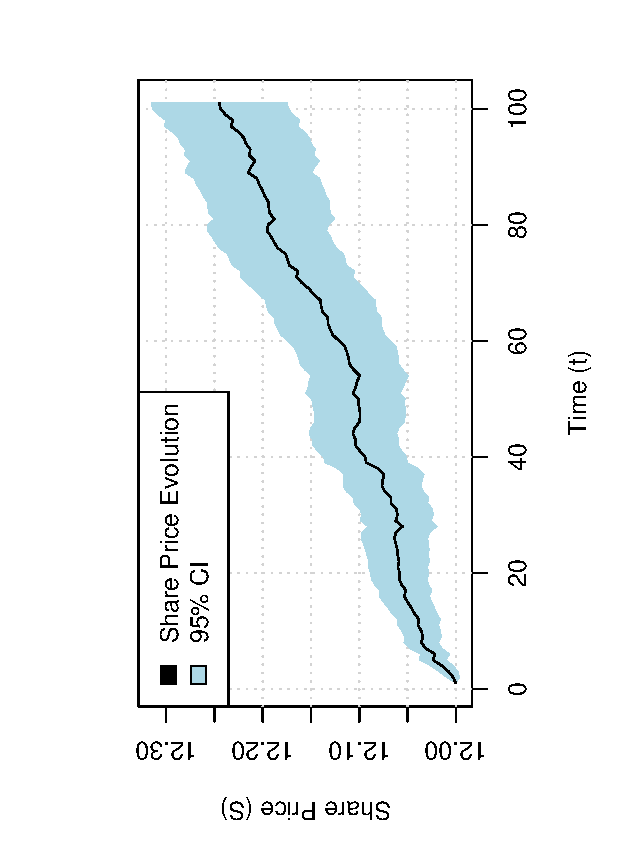
\includegraphics[scale=0.85,angle=-90]{./images/pseudo/share_evo.eps}
  \caption{Share Price Evolution}
  \label{fig:share-evo}
\end{figure}

The Monte Carlo routine reports the standard deviation which can be
used to plot the confidence intervals for derived values, such as the
discounted option price at $t=0$, and the respective $\Delta$ and
$\Gamma$ sensitivities. For all results provided in
\prettyref{sec:results} the 95\% confidence intervals are reported
using the standard error defined as $s.e.=\frac{s.d.}{\sqrt{N}}$, where $N$
is the number of MC steps.

The Monte Carlo routine exposes two configuration options which
determine the approach to the random number generation. The first one
\verb=pseudo= is a logical value which switches between a pseudo
random number generator or a Sobol sequence as the underlying random
number stream for normal variates. The second one \verb=init= is also
a logical value that determines whether the random number generator
should be initialised before the MC steps. For the purpose of the
simulations described in this report, \verb=init= was set to
\verb=TRUE=, because the Monte Carlo routine is run multiple times for
different option pricing parameters. Consequently each MC run always
generates the same stream.

The \prettyref{fig:share-evo-sobol} shows the price evolution using an
underlying Sobol sequence of the lognormal model. The price evolution
is a bit more choppy, because only 100 iterations were used to
calculate the mean path. Also, this graph shows that the confidence
interval is narrower compared to \prettyref{fig:share-evo} with only
100 MC iterations. That is an order of an magnitude less than the
simulation with pseudo random numbers.

A Sobol sequence is a low discrepancy sequence with space-filling
properties. Compared to a pseudo random number this leads to a smaller
error in the Monte Carlo routine. The construction of a low
discrepancy sequence implies that an empirical standard deviation of
the estimator in the Monte Carlo routine cannot be calculated, unless
those sequences are themselves randomised. Here Sobol sequences are
drawn in $N$ dimensions. One dimension for each Monte Carlo
iteration. Each dimension is scrambled to ensure that some of the
determinism is removed. The seed for the random scrambling is the same
as for the pseudo random number generation and so the sequences are
retained between different Monte Carlo runs with different
configurations.

\begin{figure}[!ht]
  \centering
  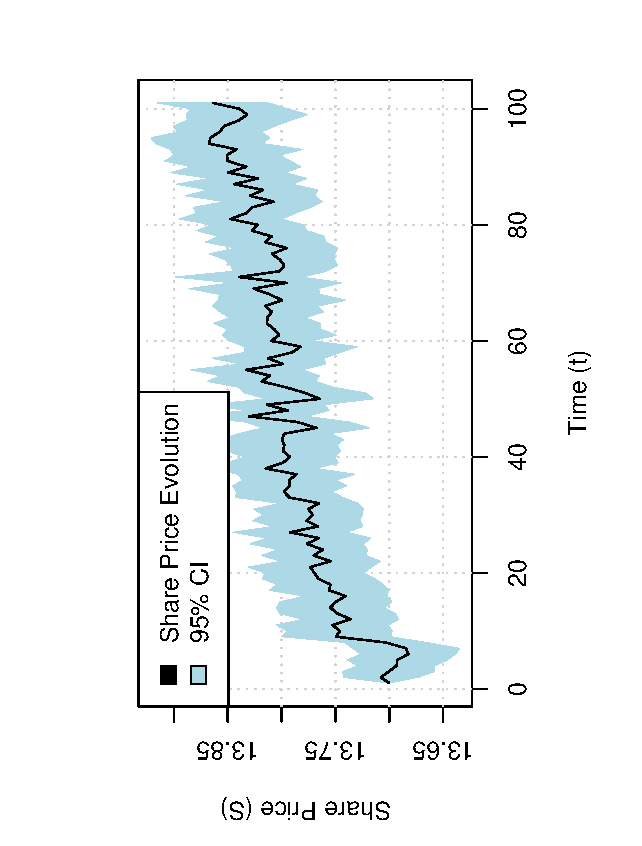
\includegraphics[scale=0.85,angle=-90]{./images/sobol/share_evo.eps}
  \caption{Share Price Evolution}
  \label{fig:share-evo-sobol}
\end{figure}


\section{Results}
\label{sec:results}

This section presents the results for five experiments conducted using
the Monte Carlo Asian Call option pricing routine.

\subsection{Volatility Bracket}
\label{sec:volatility-bracket}

\prettyref{fig:sigma1_brackets} and \prettyref{fig:sigma2_brackets}
presents two graphs plotting the price of the Asian Call option
against $\sigma_{annum}$. For this experiment the strike price is set
to $K=14$, time time-to-maturity $T=100$, the daily risk-free interest
rate $r=0.0002$, and the share price at $t=0$ is $S_{0}=12$. Plugging
$\sigma_{annum}$ into the lognormal model given in
\prettyref{eq:lognormal_model} requires a transformation into the
daily volatility using \prettyref{eq:sigma_daily}.

It can be seen that the annual volatility bracket $0\leq
\sigma_{annum} \leq 600 \%$ presents an increase in the Asian Call
option price leading up to $\sigma_{annum} \approx 5.2$ after which the
option price declines again. The maximum discounted option price at is
$C(t=0)\approx 9.3$.

\begin{figure}[!ht]
  \centering
  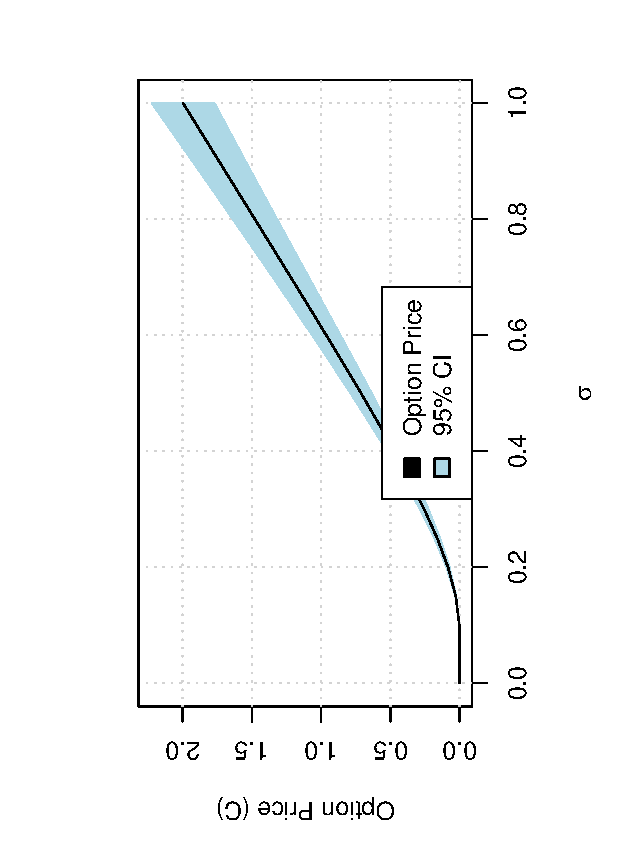
\includegraphics[scale=0.85,angle=-90]{./images/pseudo/priceOptionSigma100.eps}
  \caption{Asian Call option against $0\leq \sigma_{annum} \leq 100 \%$}
  \label{fig:sigma1_brackets}
\end{figure}

\begin{figure}[!ht]
  \centering
  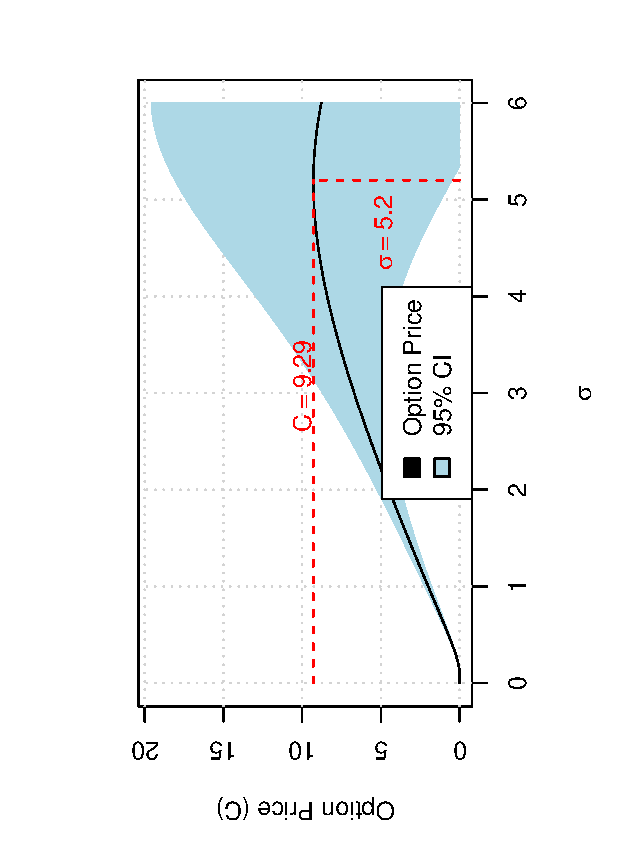
\includegraphics[scale=0.85,angle=-90]{./images/pseudo/priceOptionSigma600.eps}
  \caption{Asian Call option against $0\leq \sigma_{annum} \leq 600 \%$}
  \label{fig:sigma2_brackets}
\end{figure}

\subsection{Option Price}
\label{sec:option-price}

\prettyref{fig:option-share-price} shows the plot of the Asian Call
option price against the share price on the interval $0 \le S_{0}
\leq K$.

As expected, the option price is $0$ leading up to $S_{0} \approx 10$
after which it slowly increases to $S_{0} \approx 12$ and then
increasing linearly in $S_{0}$. The rate of change is better captured
in the $\Delta$ sensitivity plot \prettyref{fig:delta-share} in the
next section.

\begin{figure}[!ht]
  \centering
  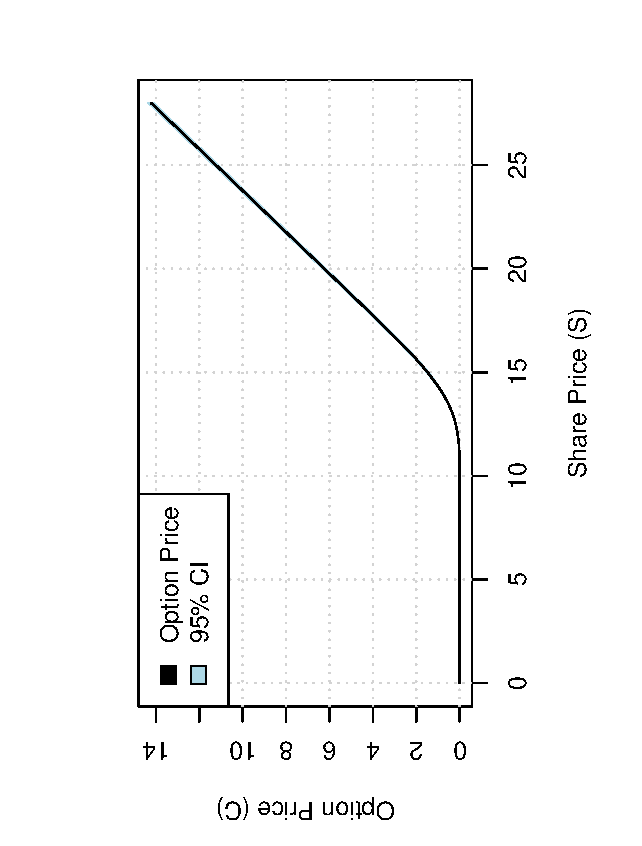
\includegraphics[scale=0.85,angle=-90]{./images/pseudo/option_share.eps}
  \caption{Asian Call option against the Share price}
  \label{fig:option-share-price}
\end{figure}

\subsection{Option Price Sensitivities}
\label{sec:opti-price-sens}

This section shows the plots of the Asian Call option sensitivities
$\Delta$ and $\Gamma$.

$\Delta$ is defined as the rate of change of the option price with
respect to the underlying share price (or more generally the
underlying asset).

Approximately in the interval of $10 \leq S_{0} \le 18$ the rate of
change is sub-linear before it reaches a value of $\Delta=1$ (see
\prettyref{fig:delta-share}). The European Call option sensitivity
$\Delta$ closely approximates the one for the Asian Call option price.

\begin{figure}[!ht]
  \centering
  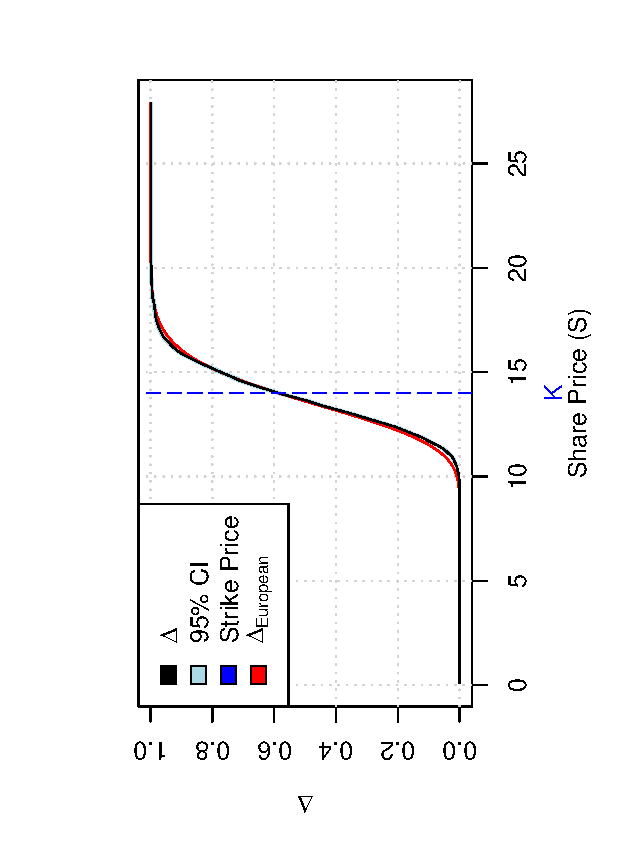
\includegraphics[scale=0.85,angle=-90]{./images/pseudo/delta_share.eps}
  \caption{Asian Call option $\Delta$ against the Share price at $t=0$}
  \label{fig:delta-share}
\end{figure}

The gamma sensitivity shown in \prettyref{fig:gamma-share} is a
little choppy, because the variability induced through the random
numbers is most pronounced in the second partial derivative of the
option price with respect to the share price. Here, the analytical
form of the European call option gamma approximates the Asian Call
option one, too.

Hedging techniques purely based on the delta sensitivity introduces
uncertainty because it measures the rate of change of the option price
to the share price (i.e., the slope), while gamma measures the
curvature of the relationship of the option price and the stock
price. So when gamma is small the call/share price relationship tends
to be linear, whereas a large gamma value implies a more pronounced
curvature of the relationship. Consequently, the larger the gamma
value is, the higher the hedging frequency ought to be in order to
maintain a delta-neutral position.

\begin{figure}[!ht]
  \centering
  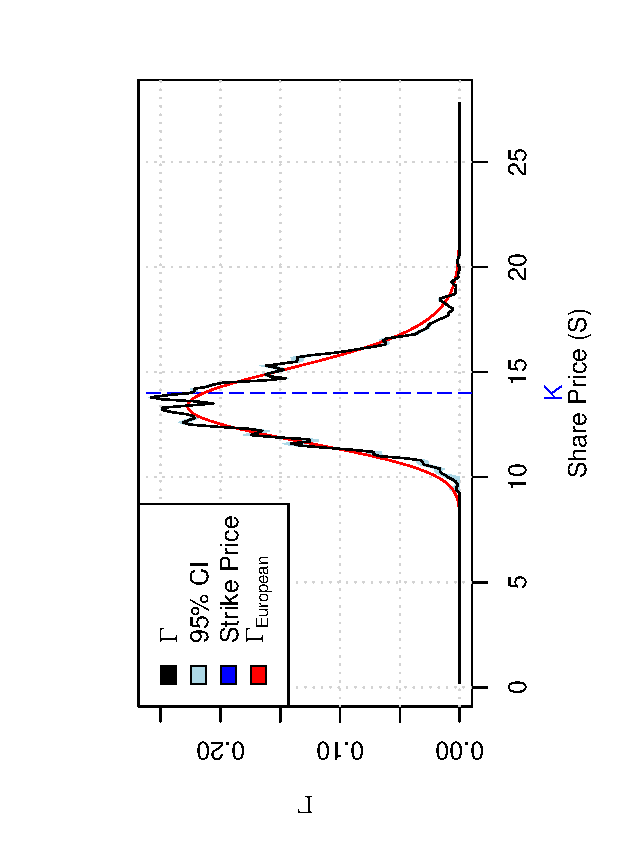
\includegraphics[scale=0.85,angle=-90]{./images/pseudo/gamma_share.eps}
  \caption{Asian Call option $\Gamma$ against the Share price at $t=0$}
  \label{fig:gamma-share}
\end{figure}

The delta and gamma values were calculated using the
central-difference scheme, i.e.,

\begin{equation}
  \label{eq:central-diff}
  f'(x) = \frac{f(x+h)-f(x-h)}{2h}
\end{equation}

Since no boundary conditions are given, each derivative requires
$f(x+h)$ and $f(x-h)$ to be defined via Monte Carlo simulation. For
the sensitivity simulation the step size of the share price was set to
$h=0.1$, i.e., an increase of 10 cent per Monte Carlo simulation.

Since 2000 Monte Carlo iterations for each data point on the graphs
was performed, the 95\% confidence interval in the sensitivity plots
is very narrow.

\section{Simulation Results for Sobol Sequences}
\label{sec:simul-results-sobol}

This section just shows the results obtained using scrambled Sobol
sequences as the underlying stream for Normal random number
generation. The curvature in the option price to share price plot is a
lot less pronounced and therefore the Delta and Gamma are curves are
narrower. I'm not sure why this is the case. The configuration used
for this setup was

\begin{verbatim}
S0 <- 13.7
K <- 14
S.min <- 0
S.max <- 2 * K
S.step <- 0.1
r <- 0.0002
sigma <- 0.013
sigma.min <- 0
sigma.step <- 0.05
T <- 100
l <- 22
reps <- 100
seed <- 123574903
pseudoRnd <- FALSE
euro <- TRUE
\end{verbatim}

\begin{figure}[!ht]
  \centering
  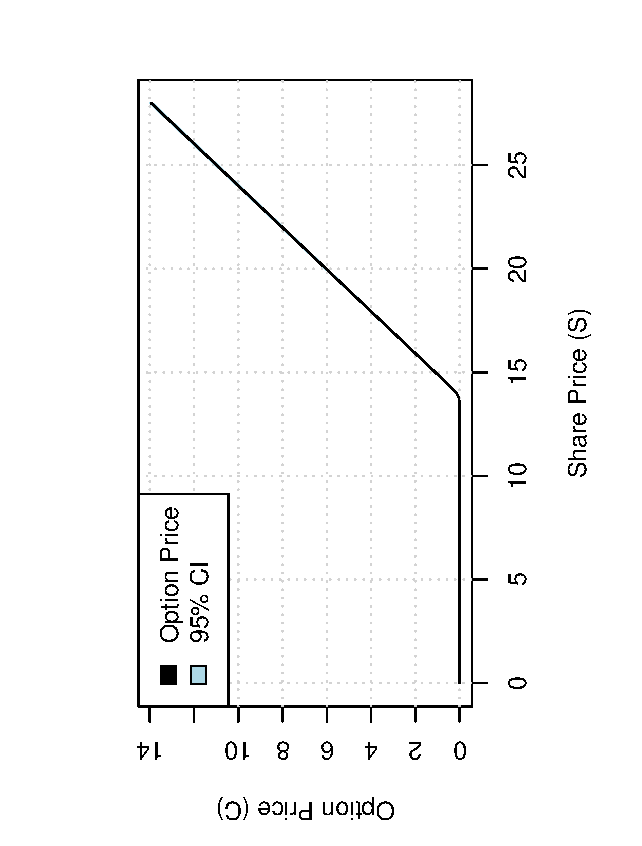
\includegraphics[scale=0.85,angle=-90]{./images/sobol/option_share.eps}
  \caption{Asian Call option against the Share price using Sobol Sequences}
  \label{fig:option-share-price-sobol}
\end{figure}
\begin{figure}[!ht]
  \centering
  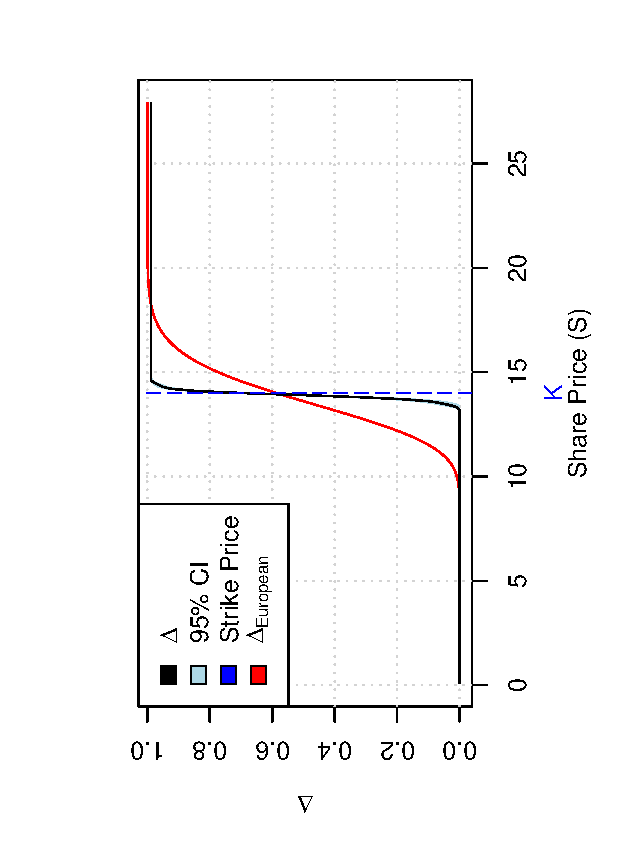
\includegraphics[scale=0.85,angle=-90]{./images/sobol/delta_share.eps}
  \caption{Asian Call option $\Delta$ against the Share price at $t=0$
  using Sobol sequences}
  \label{fig:delta-share-sobol}
\end{figure}
\begin{figure}[!ht]
  \centering
  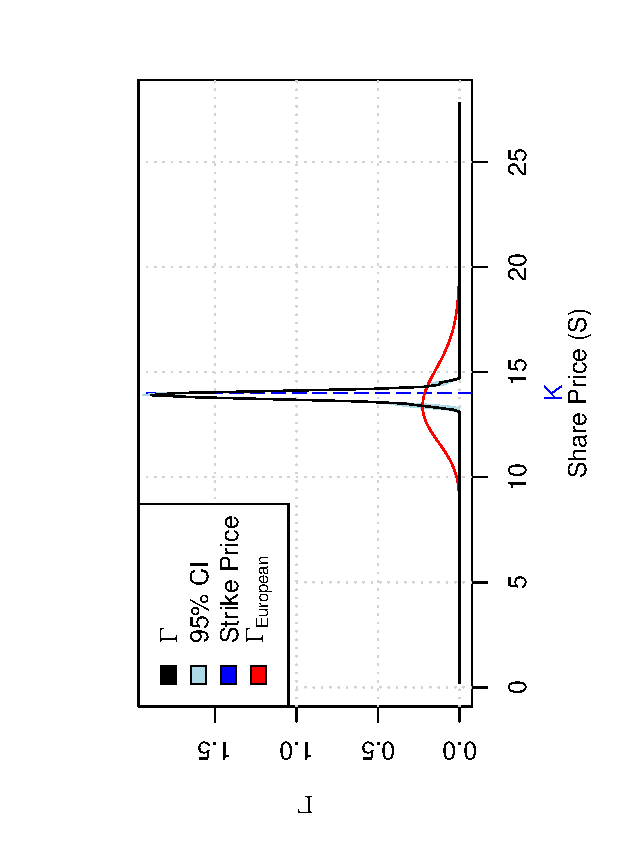
\includegraphics[scale=0.85,angle=-90]{./images/sobol/gamma_share.eps}
  \caption{Asian Call option $\Gamma$ against the Share price at $t=0$
  using Sobol sequences}
  \label{fig:gamma-share-sobol}
\end{figure}
\begin{figure}[!ht]
  \centering
  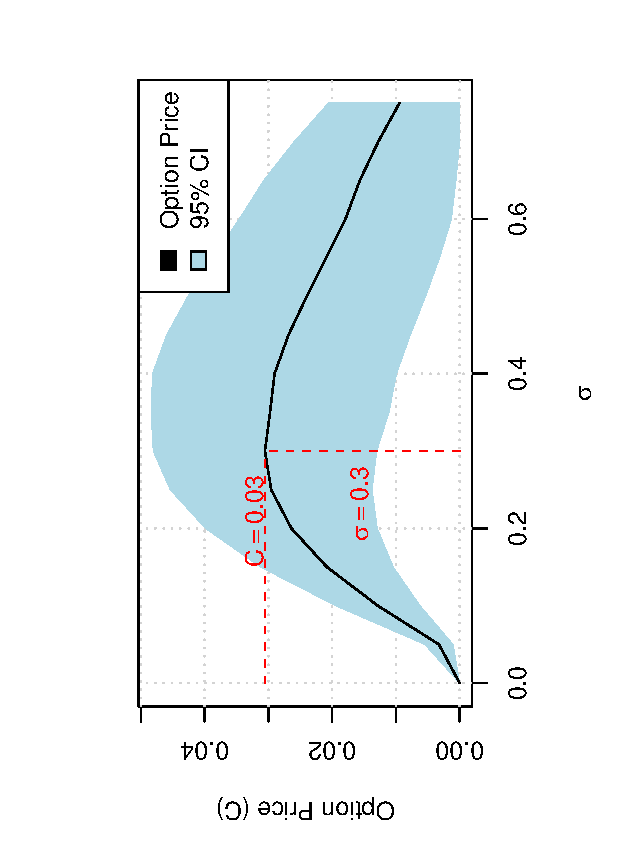
\includegraphics[scale=0.85,angle=-90]{./images/sobol/priceOptionSigma75.eps}
  \caption{Asian Call option against $0\leq \sigma_{annum} \leq 100
    \%$ using Sobol sequences}
  \label{fig:sigma_brackets-sobol}
\end{figure}

\end{document}

%%% Local Variables:
%%% mode: latex
%%% TeX-master: t
%%% End:
